\section{Исследование управляемости}

Рассмотрим систему $\dot{x} = Ax + Bu$, где 
\begin{equation}
    \begin{array}{cc}
        A = \begin{bmatrix}
            5 & -2 & 8 \\
            4 & -3 & 4 \\
            -4 & 0 & -7
        \end{bmatrix}, &
        B = \begin{bmatrix}
            -7 \\
            -5 \\
            7
        \end{bmatrix}
    \end{array}
\end{equation}

\subsection{Управляемость системы}
\subsubsection{Матрица управляемости}
Найдем матрицу управляемости $U = [B, AB, A^2B]$: 
\begin{equation}
    U = \begin{bmatrix} 
        \begin{array}{c|c|c}
            \begin{bmatrix}
                -7 \\
                -5 \\
                7
            \end{bmatrix} & 
            \begin{bmatrix}
                5 & -2 & 8 \\
                4 & -3 & 4 \\
                -4 & 0 & -7
            \end{bmatrix} \times 
            \begin{bmatrix}
                -7 \\
                -5 \\
                7
            \end{bmatrix} &
            \begin{bmatrix}
                5 & -2 & 8 \\
                4 & -3 & 4 \\
                -4 & 0 & -7
            \end{bmatrix}^2 \times
            \begin{bmatrix}
                -7 \\
                -5 \\
                7
            \end{bmatrix}
        \end{array}   
    \end{bmatrix}
\end{equation}
\begin{equation}
    U = \begin{bmatrix}
        -7 & 31 & -43 \\
        -5 & 15 & -5 \\
        7 & -21 & 23 \\
    \end{bmatrix}
\end{equation}
Определим ранг матрицы управляемости:
\begin{equation}
    \text{rank}(U) = 3
\end{equation}
Так как ранг матрицы управляемости равен порядку системы, то система является полностью управляемой согласно критерию Калмана.

\subsubsection{Управляемость собственных значений}
Найдем спектр матрицы $A$:
\begin{equation}
    \sigma(A) = \{-3, -1-2j, -1+2j\}
\end{equation}

Для каждого собственного значения найдем матрицу Хаутуса $H_i = \begin{bmatrix} A - \lambda_i I & B \end{bmatrix}$ и определим ее ранг:
\begin{enumerate}
    \item $\lambda_1 = -3$: $H_1 = \begin{bmatrix}
        8 & -2 & 8 & -7\\
        4 & 0 & 4 & -5 \\
        -4 & 0 & -4 & 7
    \end{bmatrix}$, $\text{rank}(H_1) = 3$, собственное значение управляемо.
    \item $\lambda_2 = -1-2j$: $H_2 = \begin{bmatrix}
        6+2j & -2 & 8 & -7\\
        4 & -2+2j & 4 & -5 \\
        -4 & 0 & -6+2j & 7
    \end{bmatrix}$, $\text{rank}(H_2) = 3$, собственное значение управляемо.
    \item $\lambda_3 = -1+2j$: $H_3 = \begin{bmatrix}
        6-2j & -2 & 8 & -7\\
        4 & -2-2j & 4 & -5 \\
        -4 & 0 & -6-2j & 7
    \end{bmatrix}$, $\text{rank}(H_3) = 3$, собственное значение управляемо.
\end{enumerate}
Так как выше было показано, что система является полностью управляемой, то каждое собственное значение матрицы $A$ является управляемым. 

\subsubsection{Диагональная форма системы}
Найдем диагональную форму системы, заменив базис на базис из собственных векторов матрицы $A$:
\begin{equation}
    \dot{\hat{x}} = P^{-1}AP\hat{x} + P^{-1}Bu
\end{equation}
Где $P$ -- матрица собственных векторов матрицы $A$. 
Найдем собственные векторы матрицы $A$:
\begin{equation}
    \begin{array}{ccc}
        v_1 = \begin{bmatrix} -1 \\ 0 \\ 1 \end{bmatrix} &
        v_2 = \begin{bmatrix} -3+j \\ -2 \\ 2 \end{bmatrix} &
        v_3 = \begin{bmatrix} -3-j \\ -2 \\ 2 \end{bmatrix} 
    \end{array}
\end{equation}
Тогда матрица $P$:
\begin{equation}
    P = \begin{bmatrix}
        -1 & -3+j & -3-j \\
        0 & -2 & -2 \\
        1 & 2 & 2
    \end{bmatrix}
\end{equation}
Система преобразуется к виду:
\begin{equation}
    \dot{\hat{x}} = \begin{bmatrix}
        -3 & 0 & 0 \\
        0 & -1-2j & 0 \\
        0 & 0 & -1+2j
    \end{bmatrix} \hat{x} + 
    \begin{bmatrix}
        2 \\
        \frac{5 - 5j}{4} \\ 
        \frac{5 + 5j}{4}
    \end{bmatrix} u
\end{equation}
Так как все элементы $P^{-1}B$ не равны нулю, то система является полностью управляемой, каждая мода системы управляема.

\subsection{Грамиан управляемости}
Найдем грамиан управляемости $P(t_1)$:
\begin{equation}
    P(t_1) = \int_{0}^{t_1} e^{At}BB^Te^{A^Tt}dt
\end{equation}
Вычислим грамиан управляемости для $t_1 = 3$ с помощью функции \texttt{gram}: 
\begin{equation}
    P(3) = \begin{bmatrix}
        18.12 & 10.97 & -11.64 \\ 
        10.97 & 7.48 & -8.48 \\ 
        -11.64 & -8.48 & 10.14 \\ 
    \end{bmatrix}
\end{equation}
Найдем собственные числа Грамиана управляемости: 
\begin{equation}
    \sigma(P(3)) = \{ 0.05, 1.94, 33.74 \}
\end{equation}
Все собственные числа Грамиана управляемости положительны, что говорит о том, что система является управляемой.


\subsection{Управление системой}
Найдем управление $u(t)$, которое будет переводить систему из состояния $x(0) = 0$ в состояние $x_1 = x(t_1) = \begin{bmatrix} -2 & -3 & 3 \end{bmatrix}^T$. 
\begin{equation}
    u(t) = B^Te^{A^T(t_1 - t)}P(t_1)^{-1}x_1
\end{equation}
Реализуем данное управление в MATLAB и проведем моделирование системы. 
\begin{figure}
    \centering
    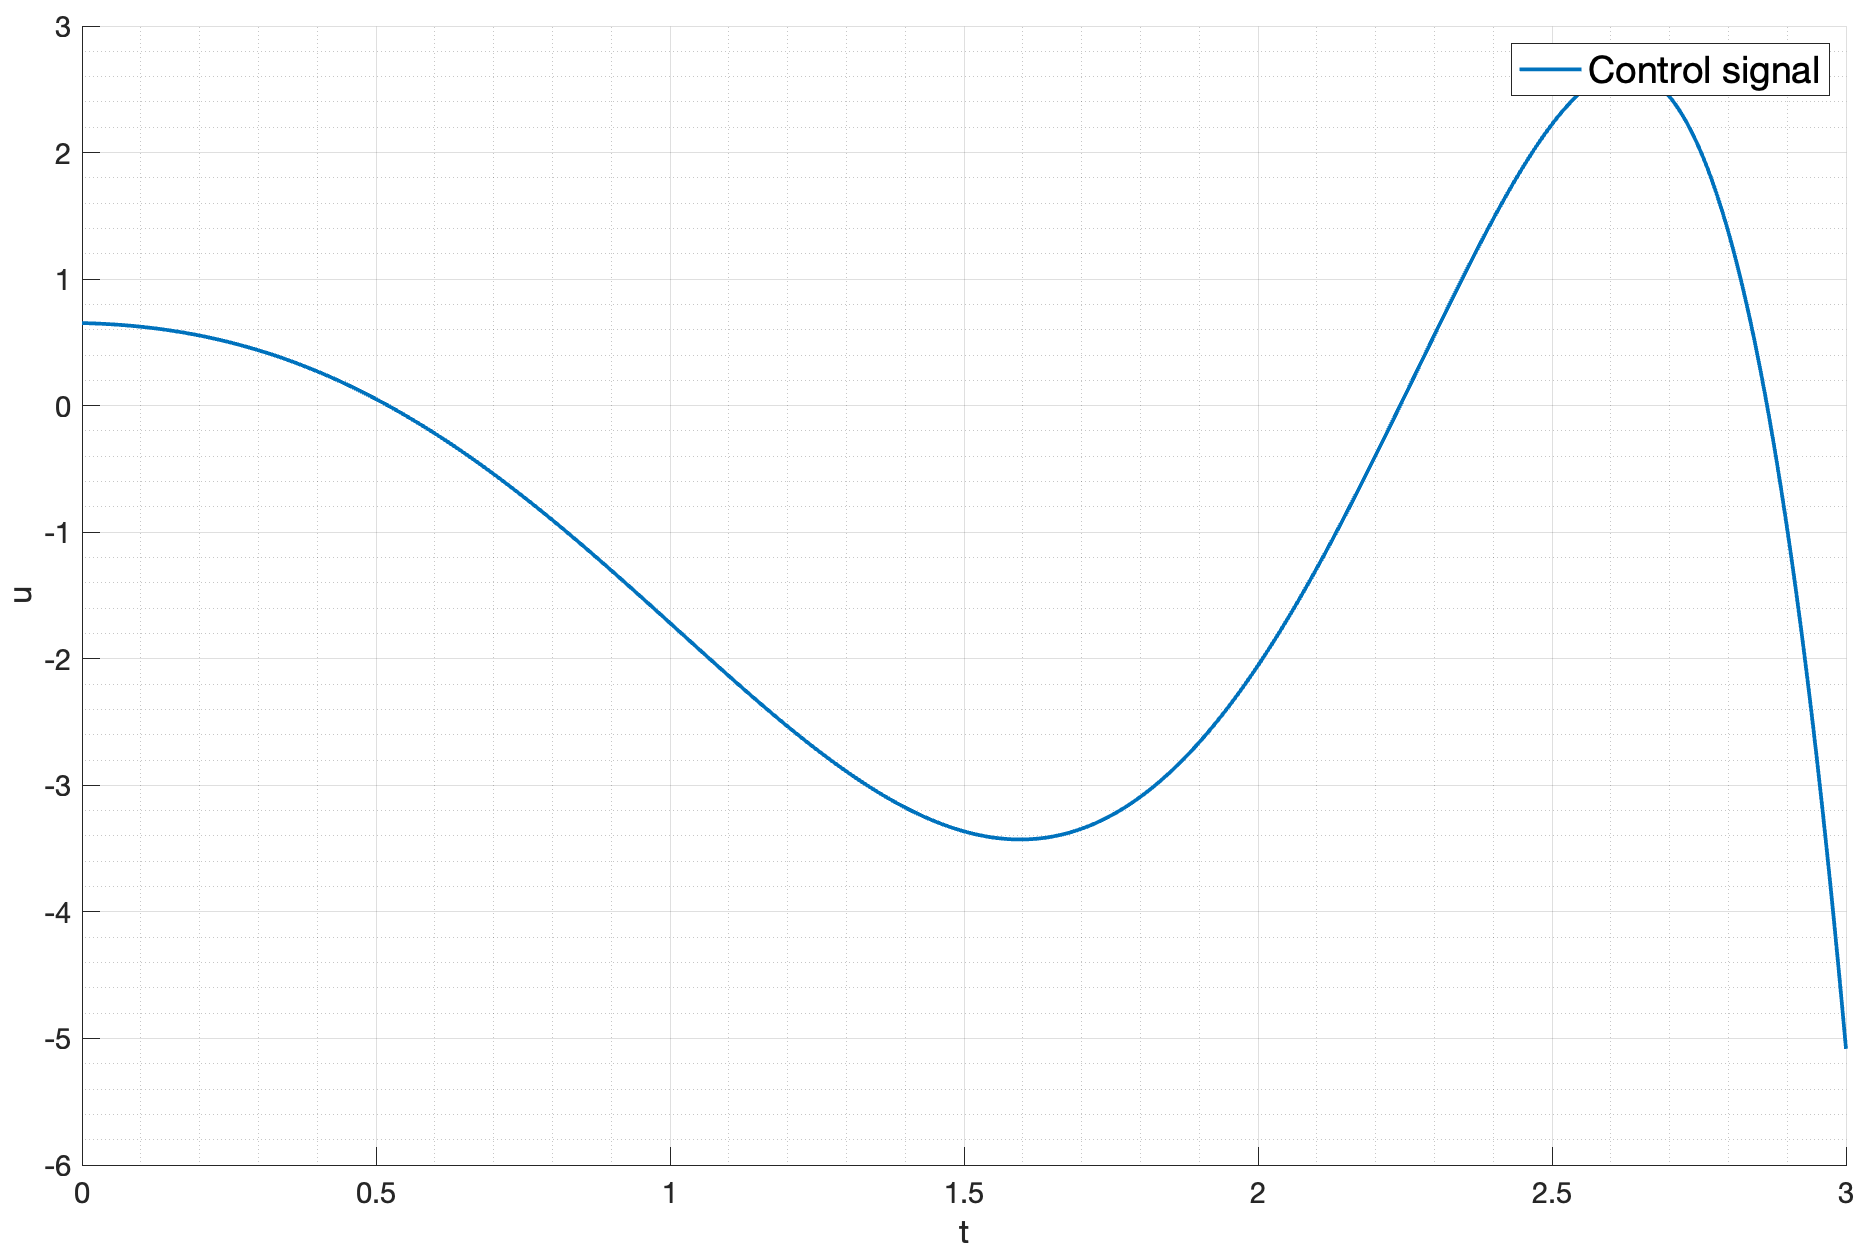
\includegraphics[width=\textwidth]{media/plots/task1_control_signal.png}
    \caption{Управление системой}
    \label{fig:task1_control_signal}
\end{figure}
На рисунке \ref{fig:task1_control_signal} изображено управление системой.
\begin{figure}
    \centering
    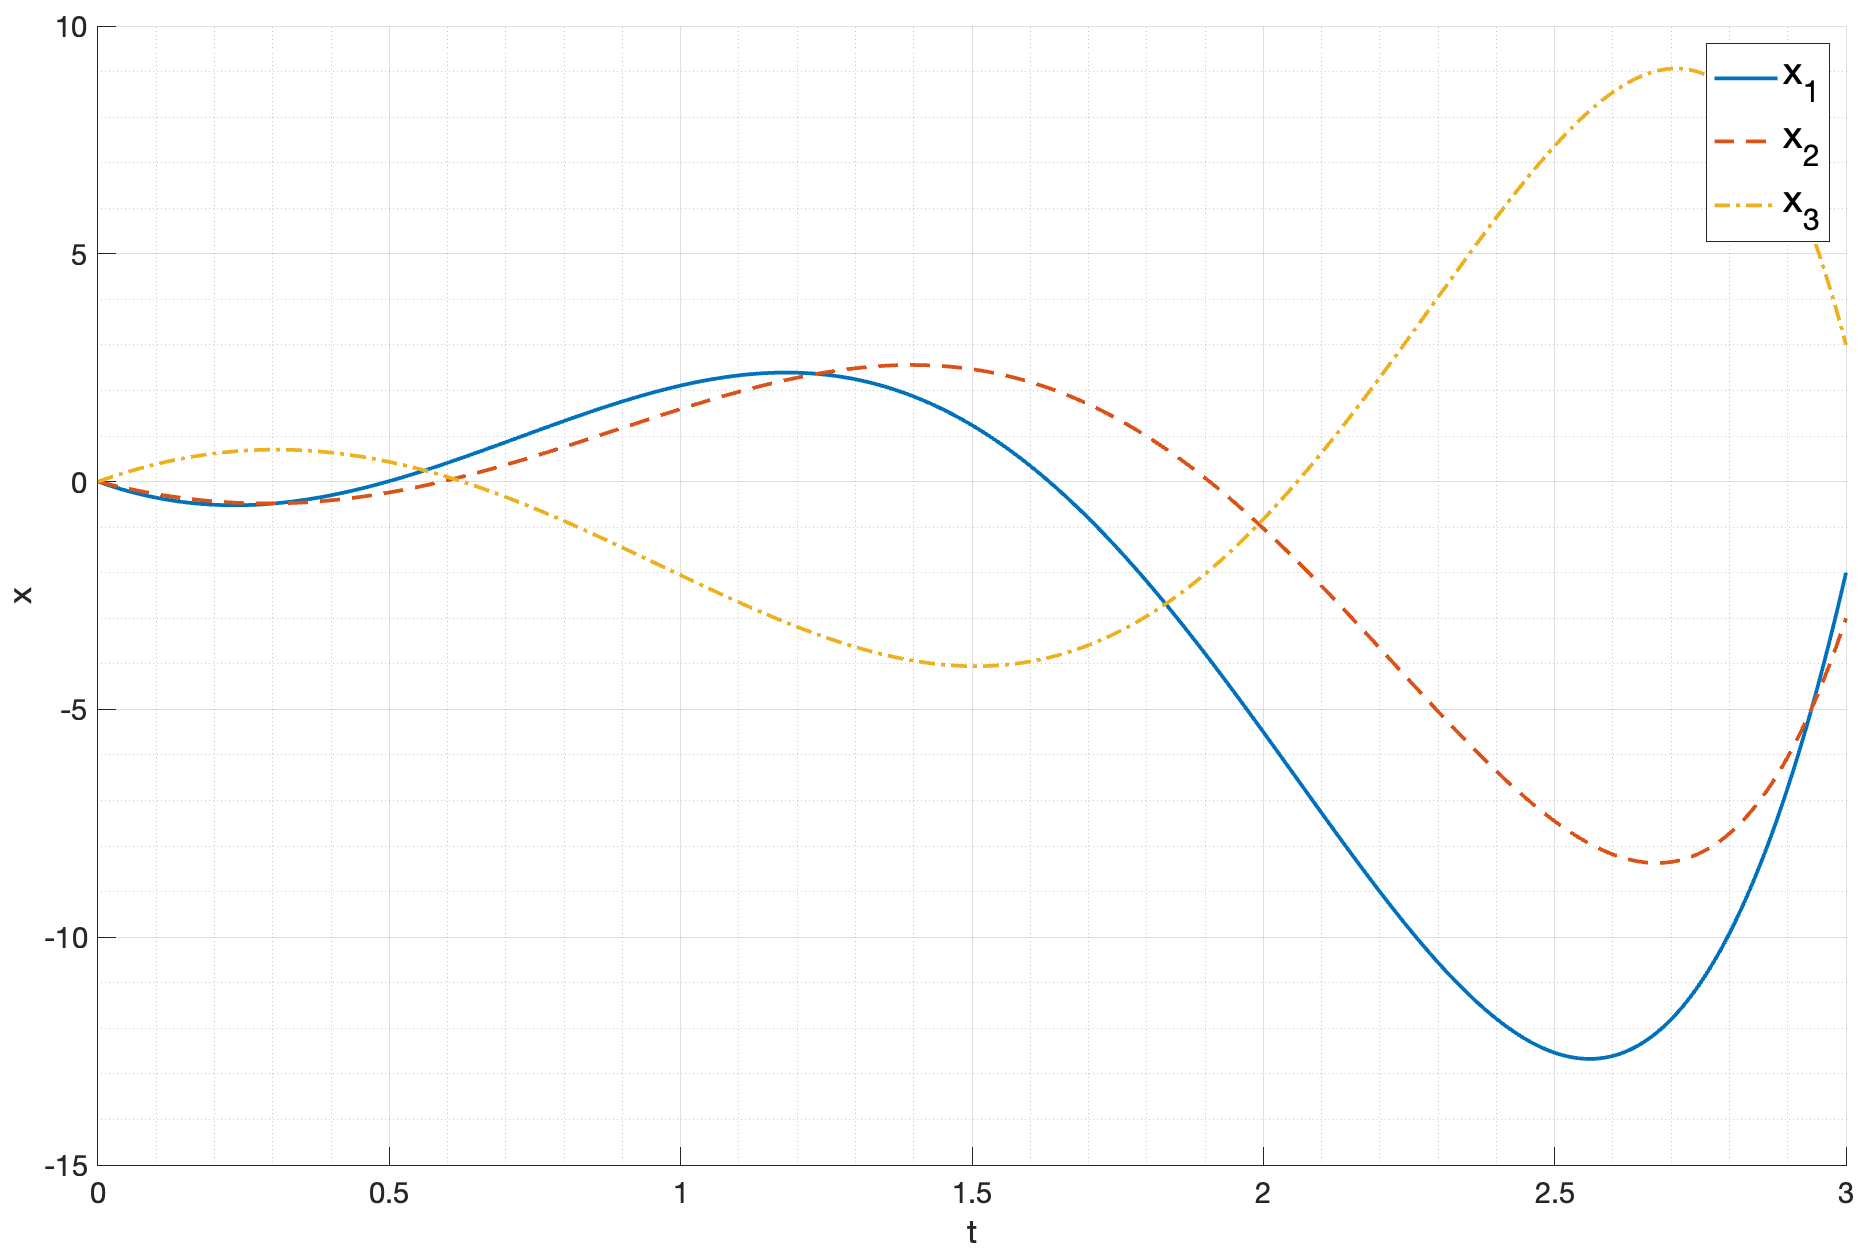
\includegraphics[width=\textwidth]{media/plots/task1_states.png}
    \caption{Состояние системы}
    \label{fig:task1_state}
\end{figure}
На рисунке \ref{fig:task1_state} изображено состояние системы.

Видно, что система управляемая в соответствии с заданным управлением и переходит в заданное состояние. 
\FloatBarrier
\subsection{Вывод}
При исследовании системы, рассматриваемой в этом заднии, удалось показать, что она является 
полностью управляемой. Это было продемонстрировано с помощью критерия Калмана, через 
управляемость собственных значений и диагональную форму системы. Также был найден грамиан 
управляемости и проверены его собственные числа. Проведено моделирование системы с управлением, 
которое переводит систему в заданное состояние. Результаты моделирования показали, что система
управляема и управление работает корректно. 
\FloatBarrier
\section{Управляемое подпространство}

Рассмотрим систему $\dot{x} = Ax + Bu$, где 
\begin{equation}
    \begin{array}{cc}
        A = \begin{bmatrix}
            5 & -2 & 8 \\
            4 & -3 & 4 \\
            -4 & 0 & -7
        \end{bmatrix}, &
        B = \begin{bmatrix}
            -1 \\
            -3 \\
            3
        \end{bmatrix}
    \end{array}
\end{equation}

\subsection{Управляемость системы}
\subsubsection{Матрица управляемости}
Найдем матрицу управляемости $U = [B, AB, A^2B]$:
\begin{equation}
    U = \begin{bmatrix} 
        \begin{array}{c|c|c}
            \begin{bmatrix}
                -1 \\
                -3 \\
                3
            \end{bmatrix} & 
            \begin{bmatrix}
                5 & -2 & 8 \\
                4 & -3 & 4 \\
                -4 & 0 & -7
            \end{bmatrix} \times 
            \begin{bmatrix}
                -1 \\
                -3 \\
                3
            \end{bmatrix} &
            \begin{bmatrix}
                5 & -2 & 8 \\
                4 & -3 & 4 \\
                -4 & 0 & -7
            \end{bmatrix}^2 \times
            \begin{bmatrix}
                -1 \\
                -3 \\
                3
            \end{bmatrix}
        \end{array}   
    \end{bmatrix}
\end{equation}
\begin{equation}
    U = \begin{bmatrix}
    -1 & 25 & -45 \\ 
    -3 & 17 & -19 \\ 
    3 & -17 & 19 \\ 
    \end{bmatrix}
\end{equation}
Определим ранг матрицы управляемости:
\begin{equation}
    \text{rank}(U) = 2
\end{equation}
Так как ранг матрицы управляемости меньше размерности матрицы $A$, система не является полностью управляемой. 

\subsubsection{Управляемость собственных значений}
Определим управляемость собственных значений матрицы $A$. Для каждого собственного значения найдем матрицу Хаутуса $H_i = \begin{bmatrix} A - \lambda_i I & B \end{bmatrix}$ и определим ее ранг:
\begin{enumerate}
    \item $\lambda_1 = -3$: $H_1 = \begin{bmatrix}
        8 & -2 & 8 & -1\\
        4 & 0 & 4 & -3 \\
        -4 & 0 & -4 & 3
    \end{bmatrix}$, $\text{rank}(H_1) = 2$, собственное значение не управляемо.
    \item $\lambda_2 = -1-2j$: $H_2 = \begin{bmatrix}
        6+2j & -2 & 8 & -1\\
        4 & -2+2j & 4 & -3 \\
        -4 & 0 & -6+2j & 3
    \end{bmatrix}$, $\text{rank}(H_2) = 3$, собственное значение управляемо.
    \item $\lambda_3 = -1+2j$: $H_3 = \begin{bmatrix}
        6-2j & -2 & 8 & -1\\
        4 & -2-2j & 4 & -3 \\
        -4 & 0 & -6-2j & 3
    \end{bmatrix}$, $\text{rank}(H_3) = 3$, собственное значение управляемо.
\end{enumerate}

\subsubsection{Диагональная форма системы}
\begin{equation}
    \dot{\hat{x}} = \begin{bmatrix}
        -3 & 0 & 0 \\
        0 & -1-2j & 0 \\
        0 & 0 & -1+2j
    \end{bmatrix} \hat{x} + 
    \begin{bmatrix}
        0 \\
        \frac{3 - 7j}{4} \\ 
        \frac{3 + 7j}{4}
    \end{bmatrix} u
\end{equation}
Первое число в векторе $P^{-1}B$ равно нулю, значит, что первое состояние системы не является управляемым. 
Результаты совпали с результатами, полученными при анализе управляемости собственных значений через матрицу Хаутуса.

\subsection{Грамиан управляемости}
Найдем грамиан управляемости $P(t_1)$:
\begin{equation}
    P(t_1) = \int_{0}^{t_1} e^{At}BB^Te^{A^Tt}dt
\end{equation}
Вычислим грамиан управляемости для $t_1 = 3$ с помощью функции \texttt{gram}: 
\begin{equation}
    P(3) = \begin{bmatrix}
        26.65 & 13.37 & -13.37 \\ 
        13.37 & 8.28 & -8.28 \\ 
        -13.37 & -8.28 & 8.28 \\ 
    \end{bmatrix}
\end{equation}
Найдем собственные числа Грамиана управляемости:
\begin{equation}
   \sigma(P(3)) = \{0, 2.03, 41.17 \}
\end{equation}
Первое собственное число равно нулю, что говорит о том, что Грамиан является вырожденным и система не является полностью
управляемой. Таким образом, для дальнейшего нахождения управления необходимо использовать псведообратную матрицу. 

\subsection{Управляемое подпространство}
Выясним, принадлежат ли точки $x_1'$ и $x_1''$ управляемому подпространству:
\begin{equation}
    \begin{array}{cc}
        x_1' = \begin{bmatrix}
            -2 \\
            -3 \\
            3
        \end{bmatrix}, &
        x_1'' = \begin{bmatrix}
            -3 \\
            -3 \\
            4
        \end{bmatrix}
    \end{array}
\end{equation}
Для этого можно записать расширенную матрицу управляемости $U'$ и найти ранг этой матрицы:
\begin{equation}
    U' = \begin{bmatrix}
        -1 & 25 & -45 & -2 \\
        -3 & 17 & -19 & -3 \\
        3 & -17 & 19 & 3
    \end{bmatrix}
\end{equation}
\begin{equation}
    \text{rank}(U') = 2
\end{equation}

\begin{equation}
   U'' = \begin{bmatrix}
        -1 & 25 & -45 & -3 \\
        -3 & 17 & -19 & -3 \\
        3 & -17 & 19 & 4
    \end{bmatrix}
\end{equation}
\begin{equation}
    \text{rank}(U'') = 3
\end{equation}
Таким образом, можно сделать вывод, что точка $x_1'$ принадлежит управляемому подпространству, а точка $x_1''$ не принадлежит. В дальнейшем будем обозначать $x_1'$ как $x_1$.

\subsection{Управление системой}
Найдем управление $u(t)$, которое будет переводить систему из состояния $x(0) = 0$ в состояние $x_1 = x(t_1) = \begin{bmatrix} -2 & -3 & 3 \end{bmatrix}^T$. 
\begin{equation}
    u(t) = B^Te^{A^T(t_1 - t)}P(t_1)^{-1}x_1
\end{equation}
Реализуем данное управление в MATLAB и проведем моделирование системы.  
\begin{figure}
    \centering
    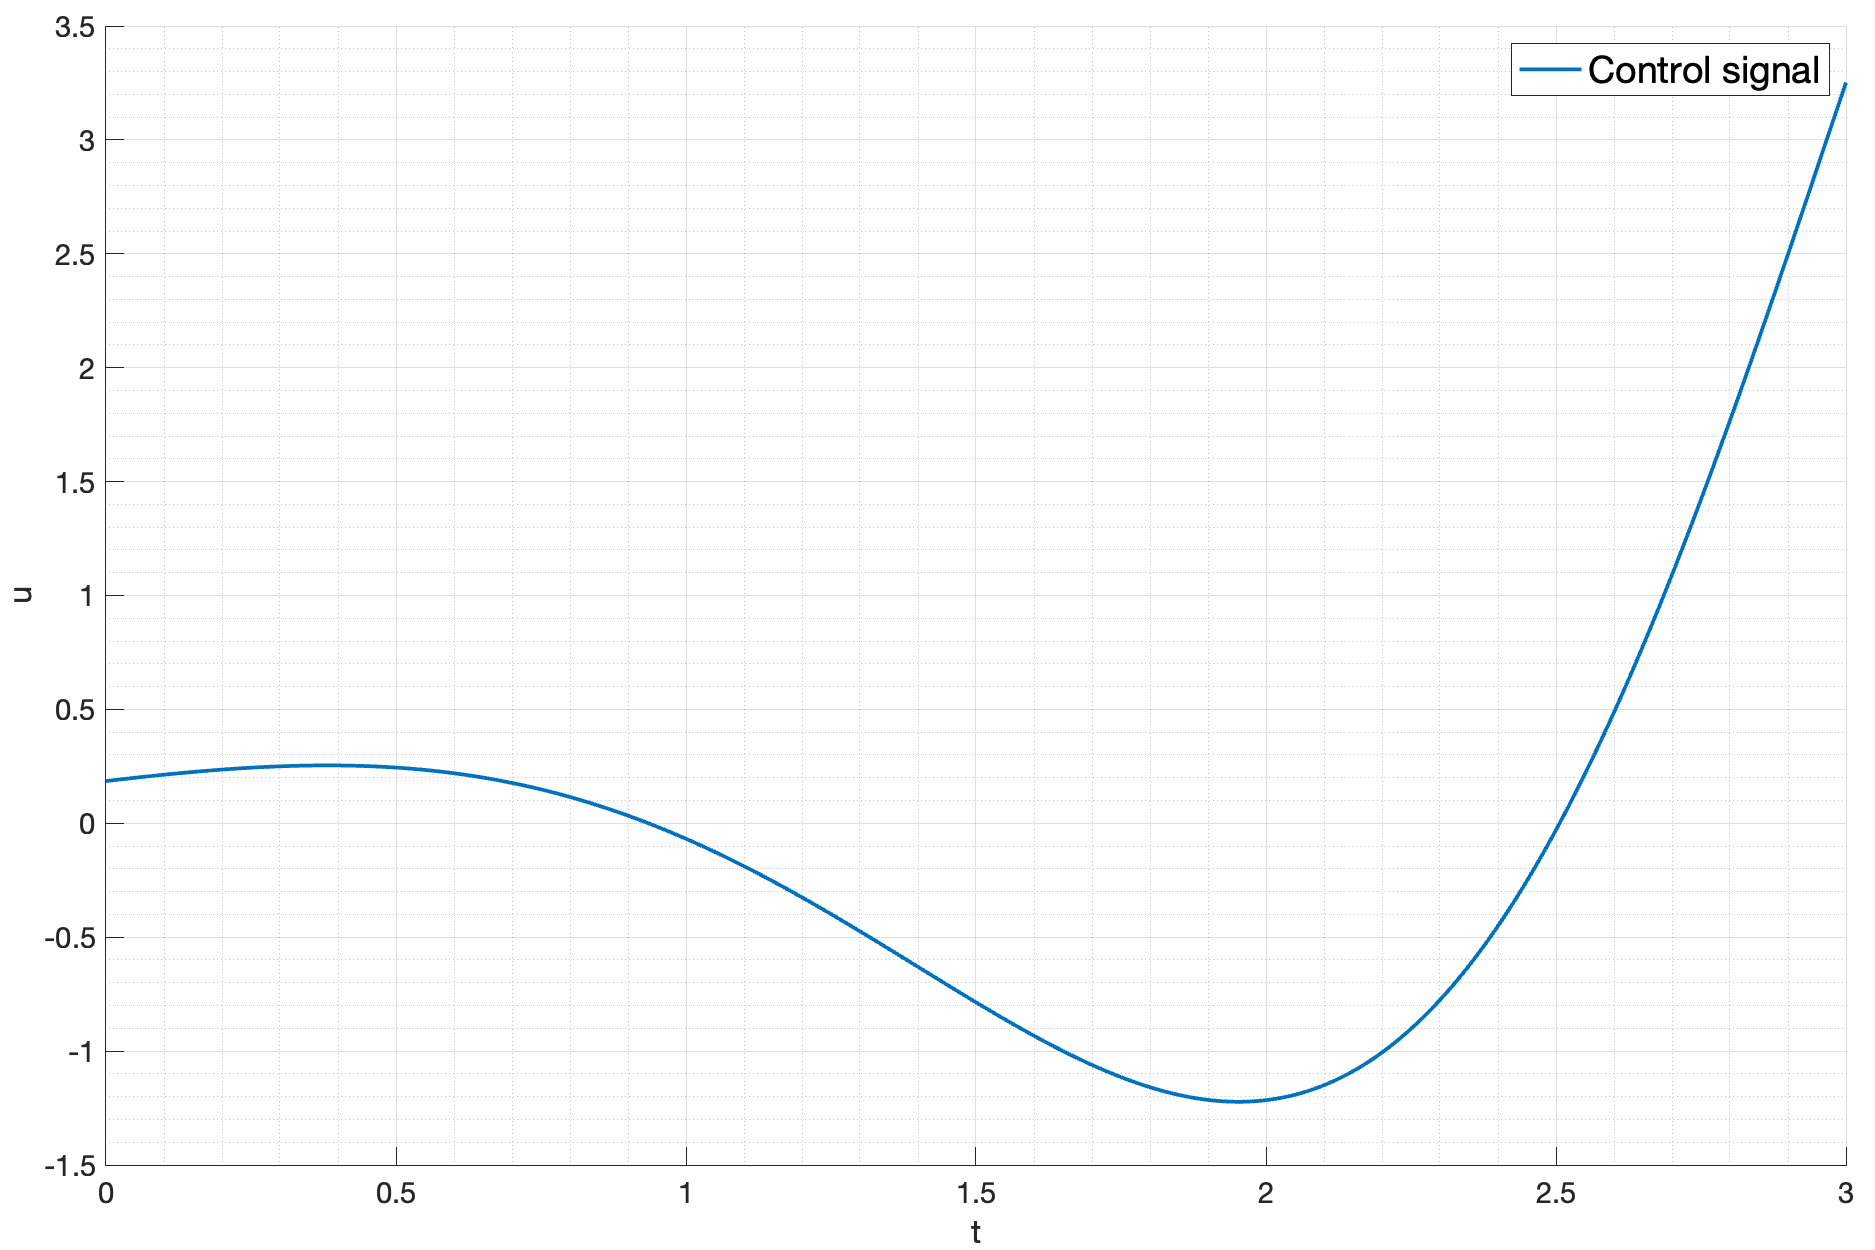
\includegraphics[width=\textwidth]{media/plots/task2_control_signal.png}
    \caption{Управление системой}
    \label{fig:task2_control_signal}
\end{figure}
На рисунке \ref{fig:task2_control_signal} изображено управление системой.
\begin{figure}
    \centering
    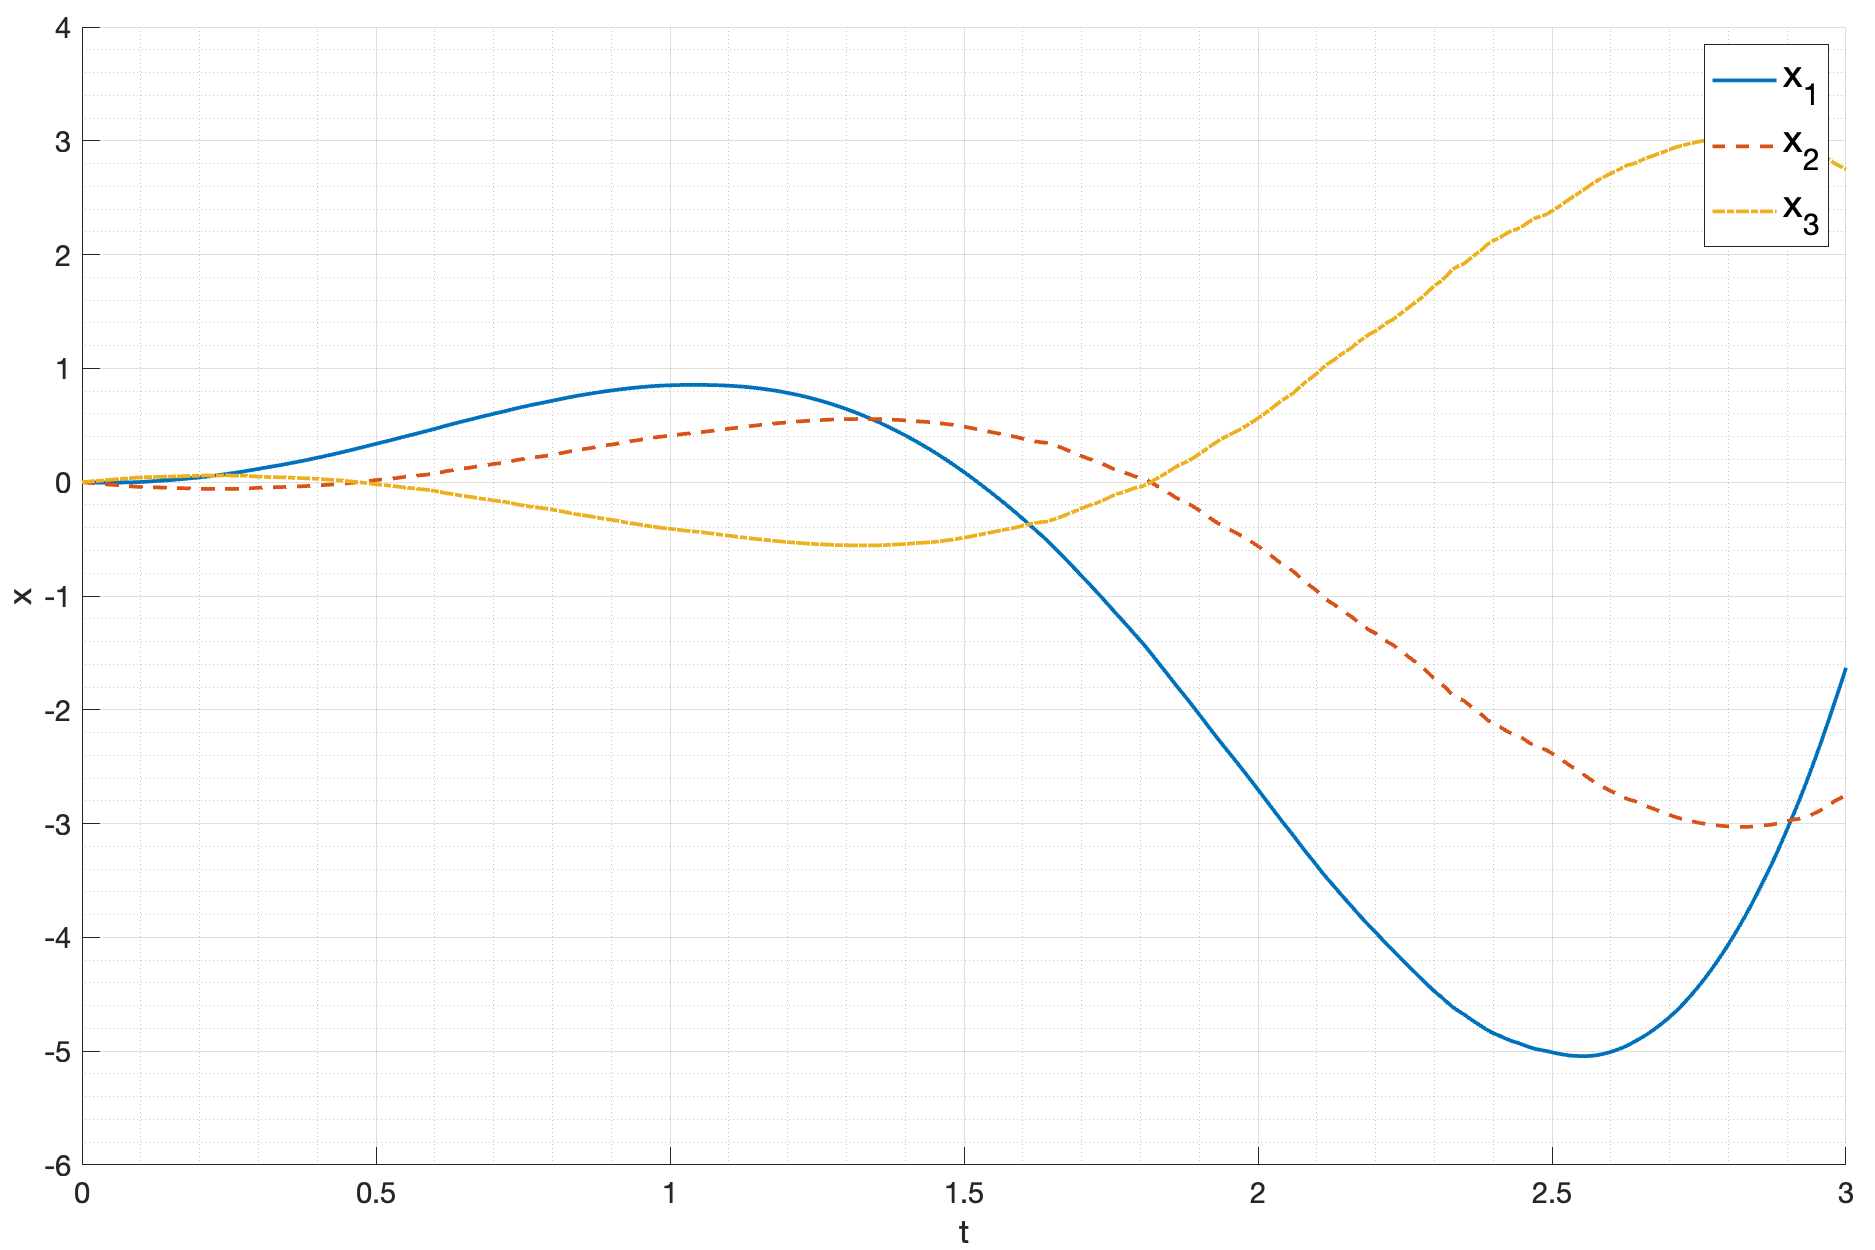
\includegraphics[width=\textwidth]{media/plots/task2_states.png}
    \caption{Состояние системы}
    \label{fig:task2_state}
\end{figure}
На рисунке \ref{fig:task2_state} изображено состояние системы.

Видно, что система управляемая в соответствии с заданным управлением и переходит в заданное состояние. 

\FloatBarrier
\subsection{Вывод}
При исследовании системы, рассматриваемой в этом задании, получилось доказать, что она 
не является полностью управляемой. Это было продемонстрировано с помощью критерия Калмана,
через управляемость собственных значений и диагональную форму системы. При этом оказалось, 
что собственное число $\lambda_1 = -3$ не является управляемым. Также был найден грамиан
управляемости и проверены его собственные числа. Одно из собственных чисел равно нулю, что
говорит о том, что система не является полностью управляемой. 

Были рассмотрены две точки $x_1'$ и $x_1''$ и проверена их принадлежность управляемому
подпространству. Точка $x_1'$ принадлежит управляемому подпространству, а точка $x_1''$ не принадлежит. 
Проведено моделирование системы с управлением, которое переводит систему в заданное состояние.
Результаты моделирования показали, что система управляема и управление работает корректно.
\FloatBarrier

\section{Выводы}
В лабораторной работе было рассмотрено вынужденное движение системы и характеристики переходных процессов.
Были рассмотрены корневые критерии качества и проведено сравнение систем с разными коэффициентами.

Моделирование систем с различными входные сигналами показало, что 
даже устойчивая система может не сходится к установившемуся значению при некоторых входных сигналах. 
Начальные условия так же влияют на поведение системы, но глобальная структура переходного процесса остается неизменной.

Результаты симуляции показали, что при увеличении максимальной величины действительной части корней 
характеристического уравнения, время переходного процесса уменьшается.
При этом, перерегулирование зависит от колебательности системы, которая пропорциональна значению $\mu = \text{max}\left|\frac{Im(\lambda)}{Re(\lambda)}\right|$.

